% Compilar con pdfLaTeX y BibTeX. Archivo principal para Overleaf: main.tex.
% El estilo visual se inspira en el artículo de referencia proporcionado.
\documentclass[10pt,a4paper,twocolumn]{article}
\usepackage[T1]{fontenc}
\usepackage[utf8]{inputenc}
\usepackage[english,spanish,es-tabla]{babel}
\usepackage[margin=1.8cm,top=1.9cm,bottom=2cm,columnsep=.65cm]{geometry}
\usepackage{newtxtext,newtxmath}
\usepackage{microtype,graphicx,booktabs,array,amsmath}
\usepackage{xcolor,titlesec,fancyhdr,caption,listings}
\usepackage{flushend}
\usepackage{cite}
\usepackage{xurl}
\usepackage[colorlinks=true,urlcolor=azul,citecolor=azul,linkcolor=azul]{hyperref}
\definecolor{vino}{HTML}{800A12}
\definecolor{azul}{HTML}{245B77}
\definecolor{gris}{HTML}{F4F4F3}
\hypersetup{pdftitle={Circuitos cuánticos reversibles: revisión y validación en Qiskit},
  pdfauthor={Brayan Vladymir Molocho Condori; Haider Alex Carpio Hermoza; Efraín Vitorino Marín}}
\newcommand{\ket}[1]{\lvert #1\rangle}
\newcommand{\bra}[1]{\langle #1\rvert}
% Generado por proyecto/experimento.py; no editar cifras manualmente.
\newcommand{\QiskitVersion}{2.6.2}
\newcommand{\ValidationCases}{552}
\newcommand{\MaxUnitaryError}{3.70e-15}
\newcommand{\MinTruthProbability}{1.000000}
\newcommand{\TwoInputRows}{AND & Toffoli & 5 & 11 & 14 \\
AND & QFT & 9 & 19 & 29 \\
NAND & Toffoli & 5 & 11 & 14 \\
NAND & QFT & 9 & 19 & 29 \\
OR & Toffoli & 5 & 11 & 16 \\
OR & QFT & 9 & 19 & 29 \\
NOR & Toffoli & 5 & 11 & 16 \\
NOR & QFT & 9 & 19 & 29 \\
XOR & Toffoli & 5 & 11 & 14 \\
XOR & QFT & 9 & 19 & 29 \\}
\newcommand{\ScalingRows}{2 & QFT & 3 & 9 & 19 \\
2 & Toffoli & 3 & 6 & 11 \\
4 & QFT & 6 & 27 & 38 \\
4 & Toffoli & 7 & 18 & 23 \\
8 & QFT & 11 & 73 & 70 \\
8 & Toffoli & 15 & 42 & 47 \\
16 & QFT & 20 & 175 & 118 \\
16 & Toffoli & 31 & 90 & 95 \\}
\newcommand{\ValidationRows}{2 & QFT & 4 & 1.000000 \\
2 & Toffoli & 4 & 1.000000 \\
4 & QFT & 16 & 1.000000 \\
4 & Toffoli & 16 & 1.000000 \\
8 & QFT & 256 & 1.000000 \\
8 & Toffoli & 256 & 1.000000 \\}

\graphicspath{{resultados/}}
\renewcommand{\thesection}{\Roman{section}}
\renewcommand{\thesubsection}{\Alph{subsection}}
\titleformat{\section}{\normalfont\normalsize\centering}{\thesection.}{.6em}{\MakeUppercase}
\titleformat{\subsection}{\normalfont\normalsize\bfseries}{\thesubsection.}{.5em}{}
\titlespacing*{\section}{0pt}{11pt}{6pt}
\titlespacing*{\subsection}{0pt}{8pt}{4pt}
\captionsetup{font=small,labelfont=bf,justification=centering}
\setlength{\parindent}{1em}
\setlength{\parskip}{2pt}
\setlength{\headheight}{14pt}
\pagestyle{fancy}
\fancyhf{}
\fancyhead[L]{\footnotesize UNSAAC · Computación Cuántica}
\fancyhead[R]{\footnotesize Avance semestral · 2026-II}
\fancyfoot[L]{\footnotesize Circuitos reversibles y Qiskit · Noviembre de 2026}
\fancyfoot[R]{\thepage}
\renewcommand{\headrulewidth}{.2pt}
\lstset{language=Python,basicstyle=\ttfamily\scriptsize,keywordstyle=\color{azul}\bfseries,
  commentstyle=\color{gray},stringstyle=\color{vino},backgroundcolor=\color{gris},
  frame=single,rulecolor=\color{gray!30},breaklines=true,showstringspaces=false,
  columns=fullflexible,keepspaces=true,aboveskip=6pt,belowskip=6pt}
\begin{document}
\twocolumn[{
\noindent{\color{vino}\bfseries\large UNIVERSIDAD NACIONAL DE SAN ANTONIO ABAD DEL CUSCO}\par
\vspace{3pt}
\noindent{\small Escuela Profesional de Ingeniería Informática y de Sistemas}\par
\vspace{8pt}
\noindent\colorbox{vino}{\parbox{\dimexpr\textwidth-2\fboxsep\relax}{
  \vspace{10pt}\centering\color{white}\fontsize{19}{23}\selectfont
  CIRCUITOS CUÁNTICOS REVERSIBLES\par
  PARA FUNCIONES BOOLEANAS:\par
  REVISIÓN Y VALIDACIÓN EN QISKIT\par\vspace{10pt}}}\par
\vspace{6pt}
\begin{center}
{\itshape\small REVERSIBLE QUANTUM CIRCUITS FOR BOOLEAN FUNCTIONS: A REVIEW AND VALIDATION IN QISKIT}\par
\vspace{8pt}
{\bfseries Brayan Vladymir Molocho Condori}\textsuperscript{1}\quad
{\bfseries Haider Alex Carpio Hermoza}\textsuperscript{2}\par
{\bfseries Efraín Vitorino Marín}\textsuperscript{3}\par
\vspace{4pt}
{\small Códigos: \textsuperscript{1}164244; \textsuperscript{2}164563; \textsuperscript{3}160337.\par
Universidad Nacional de San Antonio Abad del Cusco, Cusco, Perú.\par
Asignatura: Computación Cuántica (IF460AIN). Docente: Raúl Huillca Huallparimachi.\par
Semestre 2026-II · Avance del proyecto · Noviembre de 2026.}
\end{center}\vspace{3pt}
}]

\noindent\textbf{Resumen---}
La implementación cuántica de funciones booleanas exige preservar la información
mediante transformaciones reversibles. Este avance integra una revisión dirigida
de cuatro trabajos de 2024--2026 con una implementación reproducible en Qiskit.
Se construyen AND, NAND, OR, NOR y XOR a partir de un semisumador, usando una
realización con Toffoli y otra con la transformada cuántica de Fourier (QFT).
Las dos familias se verifican con 40 casos de tablas de verdad y con la comparación
de sus operadores completos. Además, se validan \ValidationCases{} casos de
conteo de población y AND con 2, 4 y 8 entradas, y se compilan circuitos de hasta
16 entradas. Todas las validaciones ideales satisfacen una tolerancia de
$10^{-10}$. Para 16 entradas, el conteo mediante QFT emplea 20 qubits frente a
31 de la escalera de Toffoli, pero requiere 175 compuertas CX frente a 90.
Los resultados evidencian un compromiso entre ancho, compuertas y profundidad;
la simulación ideal realizada no permite concluir superioridad en hardware.

\smallskip\noindent\textbf{Palabras clave:} circuitos reversibles, funciones booleanas,
QFT, Toffoli, Qiskit, recursos cuánticos.

\medskip\noindent\textbf{Abstract---}
\begin{otherlanguage}{english}
Boolean functions must preserve information when implemented as reversible
quantum transformations. This progress report combines a focused review of four
papers published in 2024--2026 with a reproducible Qiskit implementation.
AND, NAND, OR, NOR and XOR are constructed from a common half-adder template,
using either Toffoli gates or the quantum Fourier transform (QFT).
Both families pass 40 truth-table cases and complete operator comparisons.
An additional \ValidationCases{} population-count and AND cases are checked for
2, 4 and 8 inputs, while circuits with up to 16 inputs are compiled.
All ideal checks meet a tolerance of $10^{-10}$. At 16 inputs, the QFT circuit
requires 20 qubits rather than the Toffoli ladder's 31, but uses 175 CX gates
instead of 90. These results expose a trade-off between width, gate count and
depth; ideal simulation alone does not establish a hardware advantage.
\end{otherlanguage}

\smallskip\noindent\textbf{Keywords:} reversible circuits, Boolean functions,
QFT, Toffoli, Qiskit, quantum resources.

\section{Introducción}
Las compuertas booleanas AND y OR convierten dos bits en uno; por sí solas no
permiten recuperar la entrada. Un circuito cuántico cerrado, en cambio, actúa
mediante un operador unitario y conserva la información. Por ello, implementar
lógica clásica en computación cuántica requiere incluir registros auxiliares o
salidas residuales que vuelvan reversible la transformación \cite{nielsen2010}.

La revisión presentada en la primera parte del proyecto identificó cuatro
enfoques: aritmética basada en QFT, composición de circuitos digitales,
síntesis mediante tablas de búsqueda y minimización visual
\cite{kaltehei2026,escanez2026,clarino2025,hajjdiab2024}.
Este avance mantiene ese tema y añade una comprobación experimental propia.
La pregunta que orienta el trabajo es: \emph{¿cómo cambian los recursos al
realizar funciones booleanas reversibles con QFT en lugar de una construcción
basada en Toffoli?}

La comparación exige distinguir el número de qubits de la cantidad de
compuertas y de la profundidad. Un circuito más estrecho puede necesitar más
interacciones; además, un resultado correcto en simulación sin ruido no es una
estimación de fidelidad física. El aporte del avance consiste en hacer explícitas
estas condiciones y enlazar el análisis bibliográfico con código ejecutable,
datos tabulares y figuras generadas desde una misma ejecución.

\section{Objetivos}
\textbf{Objetivo general.} Analizar e implementar circuitos cuánticos reversibles
para funciones booleanas, contrastando diseños basados en QFT y en Toffoli bajo
condiciones comunes de compilación.

\textbf{Objetivos específicos.} Fundamentar la reversibilidad con notación de
Dirac y matrices unitarias; organizar los cuatro antecedentes de la primera
entrega; construir y validar cinco compuertas de dos entradas; estudiar el
escalamiento de un contador QFT y una escalera AND; y documentar los recursos,
las restricciones y los pasos necesarios para reproducir los experimentos.

\section{Fundamentos teóricos}
\subsection{Estados, producto interno y producto tensorial}
Un qubit puro se escribe como
\begin{equation}
\ket{\psi}=\alpha\ket{0}+\beta\ket{1},\qquad
\alpha,\beta\in\mathbb{C},\quad |\alpha|^2+|\beta|^2=1.
\end{equation}
Su normalización se expresa con el producto interno
$\langle\psi|\psi\rangle=1$. Los estados de la base computacional son
ortogonales: $\langle0|1\rangle=0$. Un sistema de $n$ qubits pertenece a
$(\mathbb{C}^2)^{\otimes n}$ y tiene $2^n$ amplitudes; el producto tensorial
permite construir estados como $\ket{a}\otimes\ket{b}=\ket{ab}$.
La medición de una cadena $x$ devuelve esa cadena con probabilidad
$|\langle x|\psi\rangle|^2$ \cite{nielsen2010}.

Una matriz estocástica describe transiciones de probabilidades clásicas. Una
matriz unitaria transforma amplitudes complejas y satisface $U^\dagger U=I$.
Aunque $|U_{yx}|^2$ define probabilidades de transición para entradas de la base,
reemplazar las amplitudes por probabilidades elimina las fases necesarias para
describir interferencia y superposición.

\subsection{Compuertas y reversibilidad}
Las puertas elementales utilizadas incluyen
\begin{equation}
X=\begin{pmatrix}0&1\\1&0\end{pmatrix},\qquad
H=\frac{1}{\sqrt2}\begin{pmatrix}1&1\\1&-1\end{pmatrix}.
\end{equation}
CNOT transforma $(a,b)$ en $(a,b\oplus a)$ y Toffoli transforma
$(a,b,c)$ en $(a,b,c\oplus ab)$. Una función clásica $f$ admite la inclusión
reversible $U_f\ket{x}\ket{z}=\ket{x}\ket{z\oplus f(x)}$.
También puede implementarse mediante otra permutación reversible que deje
$f(x)$ en una línea identificada y conserve información residual en las demás.
La familia de semisumadores de este proyecto utiliza esta segunda opción.
Bennett fundamenta el cómputo reversible y la eliminación de información
intermedia mediante cómputo, copia de la salida en la base computacional y
cómputo inverso \cite{bennett1973}. La copia mediante CNOT no clona un estado
cuántico arbitrario. Aquí los registros residuales no se limpian.
Barenco et al. demuestran la universalidad de puertas de un qubit y CNOT,
y estudian descomposiciones de controles múltiples \cite{barenco1995}; esto
respalda comparar circuitos transpilados a una base común.

\subsection{Transformada cuántica de Fourier}
Para $M=2^m$, la QFT se define como
\begin{equation}
F_M\ket{t}=\frac{1}{\sqrt M}\sum_{k=0}^{M-1}
e^{2\pi i tk/M}\ket{k}.
\end{equation}
La suma puede realizarse mediante fases en la base de Fourier
\cite{draper2000}. Si $D_b\ket{k}=e^{2\pi i bk/M}\ket{k}$,
\begin{equation}
F_M^\dagger D_bF_M\ket{t}=\ket{t+b\bmod M}.
\label{eq:add}
\end{equation}
Para $M=4$, se necesitan dos qubits en el acumulador y un control $b$.
En Qiskit se emplea \texttt{QFTGate}, con la convención de que el qubit
de índice menor tiene menor peso binario \cite{qftdocs}.
Coppersmith estudia una QFT aproximada que omite rotaciones pequeñas
\cite{coppersmith2002}. Su informe es de 1994 y fue depositado en arXiv en
2002. Este avance utiliza QFT exacta; una aproximación requeriría medir el
error de la suma y no se beneficia automáticamente de las garantías para
factorización.

\section{Antecedentes y revisión dirigida}
\subsection{Diseño lógico mediante QFT}
Kaltehei et al. \cite{kaltehei2026} construyen una familia de compuertas con
un semisumador QFT y operaciones $X$/SWAP. Extienden el diseño a conteo de
población, del que obtienen AND y paridad. Su aporte para este proyecto es
mostrar que una plantilla aritmética permite generar varias funciones y
reducir el ancho frente a una escalera con muchos auxiliares. El beneficio en
qubits debe evaluarse junto con las compuertas de dos qubits y la profundidad.
La implementación propia adopta esa arquitectura, con una convención de
registros explícita, y obtiene sus métricas nuevamente.

\subsection{Composición de circuitos digitales}
Escanez-Exposito y Caballero-Gil \cite{escanez2026} presentan QuantumSolver
Composer, una herramienta basada en Qiskit para expresar circuitos digitales
y esquemas criptográficos mediante circuitos cuánticos. El diseño modular
facilita el aprendizaje de sumadores y de otros bloques lógicos. Su utilidad
didáctica no equivale a una optimización automática de todos los recursos.
Este antecedente motiva separar en el código la construcción de circuitos,
su verificación y la generación de resultados. No se reproducen aquí sus
cifradores ni las operaciones de reinicio empleadas en algunas construcciones.

\subsection{Síntesis LUT y fases relativas}
Clarino et al. \cite{clarino2025} explotan pares de cómputo y descomputación
en redes basadas en tablas de búsqueda (LUT). Las descomposiciones de Shannon
y Davio permiten implementar funciones con fases relativas y reducir el
conteo de puertas $T$ cuando esas fases se cancelan en el circuito completo.
El resultado depende del contexto de uso y de la estructura de la red.
Para este avance, la principal consecuencia metodológica es que verificar
solo una tabla de verdad no basta: dos circuitos pueden dar los mismos bits
y diferir en fases que afectan entradas en superposición.

\subsection{Síntesis visual Q-Map}
Hajjdiab et al. \cite{hajjdiab2024} proponen Q-Map como una técnica visual
de realización cuántica de funciones booleanas. El uso de relaciones de
álgebra booleana facilita obtener construcciones compactas para los ejemplos
considerados. El enfoque ofrece una perspectiva complementaria a las
plantillas aritméticas, aunque no sustituye una comparación de compilaciones
equivalentes. En este proyecto se usa como antecedente de minimización;
no se presenta una implementación propia del algoritmo Q-Map.

\begin{table*}[t]
\centering\small
\caption{Síntesis de los cuatro antecedentes conservados de la primera entrega.}
\label{tab:literatura}
\renewcommand{\arraystretch}{1.12}
\begin{tabular}{@{}>{\raggedright\arraybackslash}p{2.5cm}>{\raggedright\arraybackslash}p{4.1cm}>{\raggedright\arraybackslash}p{4.1cm}>{\raggedright\arraybackslash}p{5cm}@{}}
\toprule
Trabajo & Estrategia & Recursos de interés & Implicación para este avance\\
\midrule
Kaltehei et al. \cite{kaltehei2026} & Semisumador y contador mediante QFT & Qubits, CX y profundidad & Comparar el ahorro de ancho con el aumento de interacciones.\\
Escanez-Exposito y Caballero-Gil \cite{escanez2026} & Composición modular de circuitos & Costo de bloques y auxiliares & Mantener circuitos y verificaciones separados y reutilizables.\\
Clarino et al. \cite{clarino2025} & Síntesis LUT con fases relativas & Conteo $T$ y cómputo/descomputación & Verificar fases; el conteo CX no reemplaza al conteo $T$.\\
Hajjdiab et al. \cite{hajjdiab2024} & Minimización visual Q-Map & Compuertas y auxiliares & Distinguir ejemplos compactos de optimalidad general.\\
\bottomrule
\end{tabular}
\end{table*}

\subsection{Fundamentos complementarios y alcance de la comparación}
Cuccaro et al. proponen un sumador de acarreo propagado de profundidad
lineal que usa un único auxiliar \cite{cuccaro2004}. Su existencia impide
interpretar el ahorro frente a nuestra escalera AND como una superioridad
sobre toda aritmética basada en Toffoli: se trata de tareas e interfaces
que deben igualarse antes de comparar. Ese sumador no está implementado aquí.

Maslov muestra identidades que permiten usar Toffoli de fase relativa en
configuraciones específicas sin alterar la operación completa
\cite{maslov2016}. Esto complementa a Clarino: sustituir cada Toffoli de
forma aislada puede introducir fases incorrectas. Se mantienen Toffoli
exactas en la implementación y se verifican matrices completas.

Shende et al. estudian síntesis de unitarias y costo CNOT, incluyendo
restricciones de interacción entre vecinos \cite{shende2006}. Su trabajo
respalda distinguir costo lógico de costo de compilación; aquí la
conectividad es completa y no se ejecuta su algoritmo de síntesis.

\section{Metodología e implementación}
\subsection{Alcance y fuentes}
Se desarrolla un estudio comparativo de simulación ideal y compilación.
La revisión es dirigida: parte de los cuatro artículos de la entrega anterior
y contrasta sus datos editoriales con las fuentes originales. Se complementa
con ocho fuentes de fundamentos y síntesis y cuatro referencias oficiales
de Qiskit: 16 referencias en total (12 académicas y cuatro de documentación).
Las seis fuentes añadidas fundamentan decisiones y límites del experimento;
no se presentan como seis métodos implementados.
No se atribuyen al proceso búsquedas exhaustivas ni cantidades de selección
de estudios propias de una revisión sistemática no realizada.

Se consideran tres niveles: funciones de dos entradas, equivalencia de
operadores y escalamiento a $N=2,4,8,16$. Las tablas de verdad se generan
localmente, por lo que no se requiere descargar un conjunto de datos externo.
La unidad de observación es una entrada binaria aplicada a un circuito.

\subsection{Semisumadores equivalentes}
Se fijan $q_0=a$, $q_1=c$ y $q_2=b$, donde $c$ inicia en cero en las tablas.
El acumulador representa $t=a+2c$. El diseño QFT implementa
\begin{equation}
(t,b)\longmapsto(t+b\bmod4,b).
\label{eq:sumador}
\end{equation}
Con $c=0$, las salidas son $q_0=a\oplus b$ y $q_1=ab$.
La implementación alternativa aplica Toffoli con controles $q_0,q_2$ sobre
$q_1$, seguida de CNOT de $q_2$ a $q_0$. Ambas implementan la misma
permutación para los ocho estados de la base, incluidos los de $c=1$.

\begin{lstlisting}[caption={Núcleo del semisumador QFT implementado.}]
from qiskit import QuantumCircuit
from qiskit.circuit.library import QFTGate
from numpy import pi

qc = QuantumCircuit(3)
qc.append(QFTGate(2), [0, 1])
qc.cp(pi / 2, 2, 0)
qc.cp(pi, 2, 1)
qc.append(QFTGate(2).inverse(), [0, 1])
\end{lstlisting}

\begin{figure}[tb]
\centering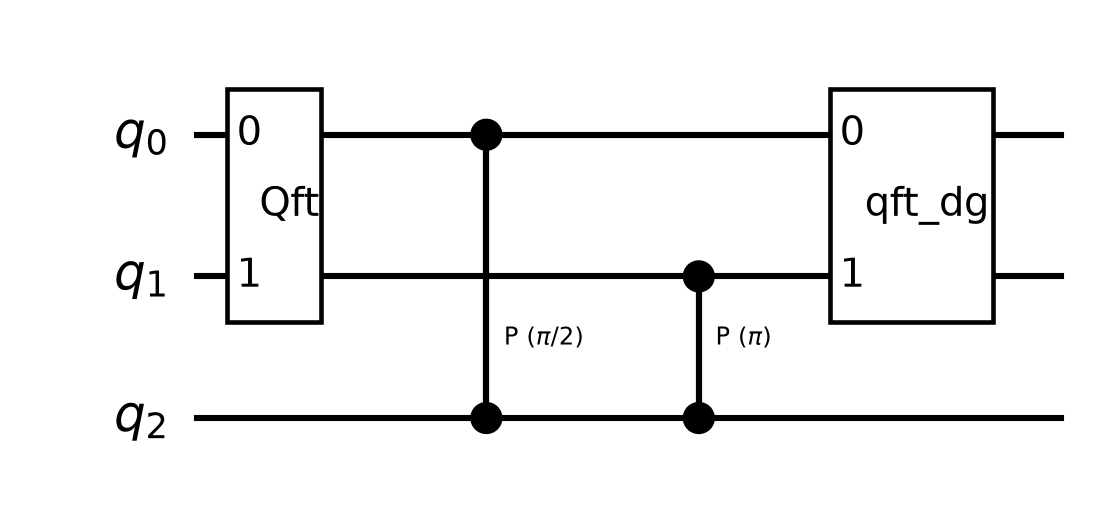
\includegraphics[height=2.6cm,width=\columnwidth,keepaspectratio]{semisumador_qft.png}\par
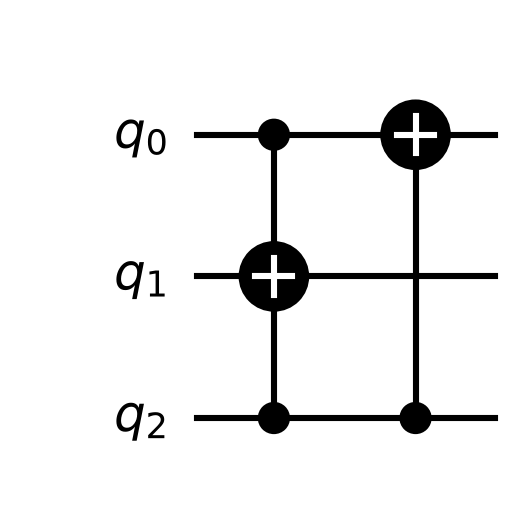
\includegraphics[height=2.6cm,width=\columnwidth,keepaspectratio]{semisumador_toffoli.png}
\caption{Semisumadores implementados: QFT (arriba) y Toffoli/CNOT (abajo).
Las figuras muestran los circuitos antes de transpilar.}
\label{fig:semisumadores}
\end{figure}

Para AND se lee $q_1$; NAND añade $X$ sobre esa salida. NOR invierte ambas
entradas antes del sumador; OR añade además $X$ en la salida. XOR intercambia
$q_0$ y $q_1$ al finalizar. Estas transformaciones se aplican a ambos diseños
para comparar la misma operación completa. Las otras líneas retienen
información residual; no se presupone que ambas entradas permanezcan intactas.

\begin{table}[tb]
\centering\small
\caption{Tabla de verdad de referencia; en los circuitos $q_1$ es la salida.}
\begin{tabular}{@{}ccccccc@{}}
\toprule
$a$ & $b$ & AND & NAND & OR & NOR & XOR\\\midrule
0&0&0&1&0&1&0\\
0&1&0&1&1&0&1\\
1&0&0&1&1&0&1\\
1&1&1&0&1&0&0\\\bottomrule
\end{tabular}
\end{table}

\subsection{Conteo de población y escalera AND}
Para $N=2^k$, el contador QFT reutiliza la primera entrada como bit menos
significativo de un acumulador de $k+1$ qubits. Añade $k$ auxiliares y mantiene
las $N-1$ entradas restantes como controles. En la base de Fourier, cada
control suma una unidad mediante fases controladas; la QFT inversa devuelve
el peso de Hamming $s=\sum_i x_i$.
Así, el ancho total es $N+k$ y las rotaciones controladas de las adiciones
son $(N-1)(k+1)$, además de las transformadas.

El bit de mayor peso vale uno exactamente cuando $s=N$, y por tanto representa
AND; el de menor peso representa la paridad. La escalera alternativa usa
$N-1$ Toffoli y $N-1$ auxiliares, para un ancho de $2N-1$ qubits. Conserva
las entradas y productos intermedios sin descomputarlos. Ambos diseños
proporcionan AND, pero sus registros residuales y sus capacidades adicionales
son distintos: el contador también entrega $s$. Por ello, en este experimento
se compara la tarea AND y los recursos, sin afirmar equivalencia de los
operadores completos de ambos diseños multientrada.

\subsection{Protocolo de validación}
Se prueban las cuatro entradas de cada compuerta en cada familia: cinco
funciones por cuatro entradas por dos diseños, es decir, 40 casos.
La simulación utiliza \texttt{Statevector} \cite{statedocs} y verifica la
probabilidad exacta del resultado esperado. Para las cinco parejas de
circuitos de tres qubits se calcula
\begin{equation}
\varepsilon=\max_{ij}|(U_{\mathrm{QFT}}-U_{\mathrm{Toffoli}})_{ij}|,
\end{equation}
además de $\max_{ij}|(U^\dagger U-I)_{ij}|$. Se adopta tolerancia $10^{-10}$.
Esta comparación incluye amplitudes y fases de los ocho estados de la base,
por lo que es más exigente que comprobar únicamente probabilidades.

Para cada diseño multientrada se exploran exhaustivamente $2^N$ entradas
cuando $N=2,4,8$: $2(4+16+256)=\ValidationCases{}$ casos.
En QFT se comprueba el conteo completo; en la escalera, AND.
Para $N=16$ se construyen y compilan los circuitos, sin simular sus
$65\,536$ entradas. Una demostración adicional prepara $H$ en $q_0$ y $q_2$,
aplica el semisumador QFT y obtiene 4096 muestras con semilla 42.
El histograma es muestreo ideal en CPU.

\subsection{Compilación y reproducibilidad}
Se usa Python 3.12 y Qiskit \QiskitVersion{}, con dependencias fijadas.
Ambas alternativas se transpilan a $\{U,\mathrm{CX}\}$, con nivel de
optimización 3, semilla 42 y conectividad completa \cite{compiledocs}.
Se indica \texttt{qubits\_initially\_zero=False}, de modo que la compilación
no suponga que las entradas lógicas son cero.
El ancho, el número de CX, la profundidad y el total de compuertas se
calculan sobre esos circuitos; la preparación y la medición se excluyen
de las tablas de recursos.

El compilador puede representar un SWAP final mediante una permutación de
las salidas. Esa permutación se registra y se utiliza al comparar el operador
compilado con el original mediante \texttt{Operator.from\_circuit}
\cite{operatordocs}. Por tanto, los conteos corresponden a circuitos con
etiquetado lógico de salidas, sin exigir que las líneas finales mantengan
un orden físico fijo. La exportación OpenQASM incluye mediciones.

\section{Resultados del avance}
\subsection{Corrección y coherencia}
Los 40 casos de tablas de verdad coinciden con las funciones esperadas.
La probabilidad mínima se redondea a \MinTruthProbability{}.
La discrepancia máxima entre las parejas de operadores y entre las versiones
compiladas y originales es \texttt{\MaxUnitaryError{}}, inferior a la
tolerancia establecida. La prueba de unitariedad también satisface esa
tolerancia. Estas verificaciones respaldan la corrección de los circuitos
ideales de tres qubits, incluidas entradas coherentes.

\begin{table}[tb]
\centering\small
\caption{Recursos propios para las cinco compuertas de dos entradas.
Todos los circuitos usan tres qubits.}
\label{tab:dos}
\begin{tabular}{@{}llrrr@{}}
\toprule
Función & Diseño & CX & Prof. & Total\\\midrule
\TwoInputRows
\bottomrule
\end{tabular}
\end{table}

La Tabla~\ref{tab:dos} muestra que la implementación QFT de esta plantilla
requiere más CX y mayor profundidad. Estos valores son resultados de la
versión y las condiciones indicadas; no se copian de los artículos.
La igualdad de recursos entre algunas funciones proviene de las simplificaciones
del compilador y del tratamiento de las permutaciones de salida.
En particular, la fila XOR evalúa la plantilla de semisumador completa;
un XOR que únicamente conserva las dos entradas y actualiza un objetivo
puede construirse con dos CNOT. No se atribuye optimalidad a la plantilla.

\begin{table}[tb]
\centering\small
\caption{Validación exhaustiva multientrada. Las probabilidades se muestran
con seis decimales; las diferencias residuales son de redondeo numérico.}
\label{tab:validacion}
\begin{tabular}{@{}rlrr@{}}
\toprule
$N$ & Diseño & Casos & Prob. mínima\\\midrule
\ValidationRows
\bottomrule
\end{tabular}
\end{table}

La Tabla~\ref{tab:validacion} recoge \ValidationCases{} verificaciones
adicionales satisfactorias. En el experimento con entradas uniformes en
superposición, medir el acumulador produce probabilidades teóricas
$P(00)=1/4$, $P(01)=1/2$ y $P(10)=1/4$: corresponden a sumar dos bits
uniformes. La Figura~\ref{fig:superposicion} contrasta esas probabilidades con
las muestras; las pequeñas diferencias provienen del muestreo finito.

\begin{figure}[tb]
\centering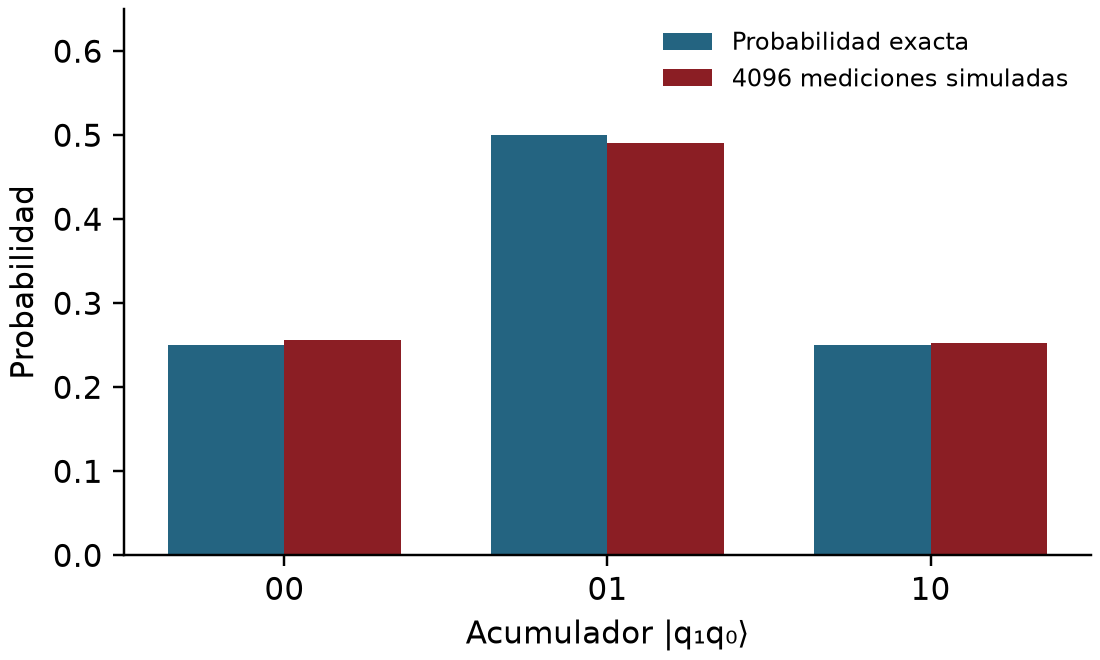
\includegraphics[width=\columnwidth]{superposicion.png}
\caption{Medición simulada del acumulador tras aplicar el semisumador QFT
a entradas en superposición. No se usó un procesador cuántico físico.}
\label{fig:superposicion}
\end{figure}

\subsection{Escalamiento de recursos}
\begin{table}[tb]
\centering\small
\caption{Recursos compilados propios para AND multientrada. QFT entrega
además el peso de Hamming; Toffoli corresponde a la escalera sin descomputación.}
\label{tab:escala}
\begin{tabular}{@{}rlrrr@{}}
\toprule
$N$ & Diseño & Qubits & CX & Prof.\\\midrule
\ScalingRows
\bottomrule
\end{tabular}
\end{table}

La Tabla~\ref{tab:escala} y la Figura~\ref{fig:recursos} muestran el compromiso
principal. Para $N=16$, el contador usa $16+\log_2 16=20$ qubits y la escalera
usa $2(16)-1=31$: la reducción es de 11 qubits, aproximadamente $35.5\%$.
En cambio, los conteos son 175 y 90 CX, respectivamente, y las profundidades
son 118 y 95. El contador reduce ancho a costa de más interacciones y capas.
Las cifras de $N=16$ describen compilación; la validación exhaustiva propia
se limita a $N\leq8$.

\begin{figure*}[t]
\centering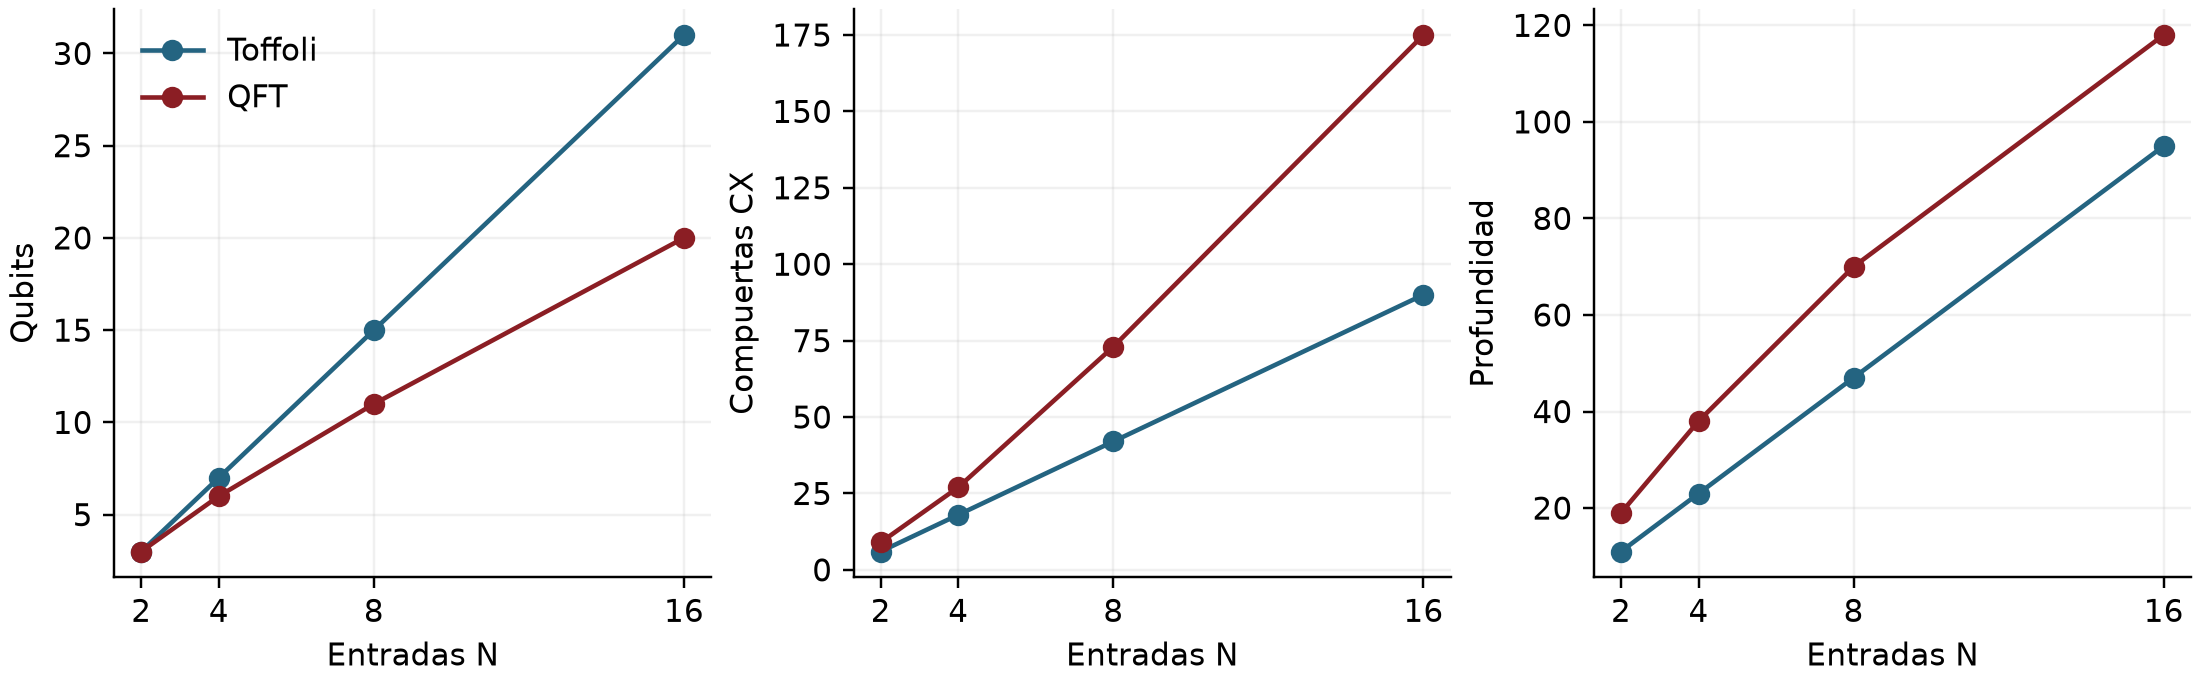
\includegraphics[width=.97\textwidth]{comparacion_recursos.png}
\caption{Comparación propia de ancho, CX y profundidad bajo una misma base
y conectividad completa. Las líneas unen los tamaños compilados; no representan
mediciones de tiempo ni de fidelidad en hardware.}
\label{fig:recursos}
\end{figure*}

\section{Discusión y limitaciones}
Los resultados concuerdan con el compromiso de recursos que motiva el diseño
QFT de la literatura: ahorrar auxiliares no garantiza reducir compuertas.
La generalización del contador añade $(N-1)(k+1)$ fases controladas y dos
transformadas de $k+1$ qubits. La escalera añade $N-1$ Toffoli y conserva
productos parciales en un registro mayor. La elección depende de la
disponibilidad de qubits y del costo físico de las interacciones.

La revisión y la experimentación cumplen funciones distintas. Los artículos
LUT y Q-Map aportan perspectivas de síntesis; las pruebas propias solo
implementan la familia de semisumadores y las dos construcciones de
escalamiento descritas. No se reproducen las ejecuciones en hardware,
los cifradores ni los bancos de pruebas de los cuatro artículos.
Asimismo, contar CX en una base de rotaciones continuas no permite inferir
directamente un conteo $T$ en un régimen tolerante a fallos.

La simulación exacta no incluye decoherencia, errores de lectura, errores
de puertas ni conectividad restringida. Un valor de probabilidad cercano
a uno demuestra consistencia matemática del modelo implementado, no
fidelidad de una QPU. En una arquitectura con acoplamientos limitados,
el enrutamiento puede introducir SWAP y modificar la comparación.
Las fases pequeñas del contador también exigen estudiar precisión o
aproximaciones antes de extrapolar a tamaños mayores.

La escalera conserva entradas y productos parciales, mientras que el contador
reutiliza una entrada y proporciona una suma. La tabla de escalamiento
compara la disponibilidad de AND como salida, no interfaces reversibles
idénticas. Una integración en un algoritmo mayor deberá especificar qué
registros deben conservarse y cuáles deben descomputarse. Exigir esa limpieza
puede modificar ancho y profundidad en ambas alternativas.

Por último, los conteos pueden variar al cambiar la versión del compilador,
el conjunto de puertas o la política de permutaciones. Las dependencias,
la configuración y las permutaciones se guardan junto con los resultados.
Las diferencias frente a cifras publicadas deben examinarse bajo esas
condiciones, en lugar de asumir que implementaciones distintas son una
reproducción literal del mismo experimento.

\section{Conclusiones y trabajo pendiente}
Se transformó el avance bibliográfico sobre circuitos reversibles en un
estudio con implementación Qiskit, validación y resultados propios.
Las cinco funciones de dos entradas pasan sus 40 casos de tablas de verdad,
y la comparación de operadores confirma que las dos realizaciones implementan
la misma transformación, incluidas sus fases. El contador y la escalera
superan además \ValidationCases{} casos exhaustivos para 2, 4 y 8 entradas.

El análisis de hasta 16 entradas demuestra que el diseño QFT ofrece un ancho
menor que la escalera considerada para $N\geq4$, pero requiere más CX y mayor profundidad
en las condiciones utilizadas. Por ello, este avance respalda una evaluación
con varias métricas y no una afirmación de ventaja general de QFT.

La siguiente etapa contempla simulación con ruido y conectividad de un
dispositivo especificado, comparación con descomposiciones MCX de pocos
auxiliares, evaluación de QFT aproximada y descomputación de registros
residuales. Cualquier resultado físico se documentará con fecha, dispositivo,
calibración y número de mediciones. Esas actividades permanecen pendientes.

\section{Material reproducible}
El código principal es \texttt{proyecto/experimento.py}; su ejecución desde
la raíz con \texttt{python -m proyecto.experimento} genera tablas CSV,
métricas JSON, diagramas, un circuito OpenQASM~3 y el archivo de macros
\texttt{resultados.tex}. El artículo incorpora esas macros y figuras para
mantener las cifras sincronizadas. El repositorio incluye instrucciones de
instalación y 12 pruebas automatizadas. El paquete de Overleaf contiene
\texttt{main.tex}, la bibliografía y todos los recursos del documento.

\clearpage
\bibliographystyle{IEEEtran}
\bibliography{referencias}
\end{document}
